\section{2024.2.27 Young diagrams}\label{4}
Some code examples of Young diagrams and tableaux using the \texttt{ytableau} package:

\begin{ytableau}
  \none[2] &  &  & \none \\
  \none[1]  &  &  &  \\
  \none & \none[1] & \none[2] & \none[3]
\end{ytableau}

\ydiagram{1,2,1}



\[
  \begin{ytableau}
    \none &  & \cdots &\\
    ~ & \none & \none & \none \\
    ~ & \none & \none & \none \\
    \vdots & \none & \none & \none \\
    x & \none & \none & \none
  \end{ytableau}
  ~+~
  \begin{ytableau}
    ~ & \none & \none & \none & \none\\
    ~ & \none & \none & \none & \none\\
    \vdots & \none & \none & \none & \none\\
    x &  &  & \cdots &
  \end{ytableau}
  ~=~
  \begin{ytableau}
    ~ & \none & \none & \none & \none\\
    ~ & \none & \none & \none & \none\\
    \vdots & \none & \none & \none & \none\\
    x & \none & \none & \none & \none\\
    ~ &  &  & \cdots &
  \end{ytableau}
\]


% 综合示例
\[
\begin{ytableau}
*(blue) a & *(yellow) b & *(green) c \\ 
*(red) 1 & 2 \\
3
\end{ytableau}
\]

% 水平对齐
\[
\begin{ytableau}
~ & ~ & ~ \\ 
~ & ~ \\
~
\end{ytableau}
\hspace{3em}
\begin{ytableau}
~ & ~ \\
~ & ~ \\
~ 
\end{ytableau}
\]

% 垂直对齐
\[
\begin{array}{c}
\begin{ytableau}
~ & ~ & ~ \\ 
~ & ~ \\
~
\end{ytableau} \\[3em]
\begin{ytableau}
~ & ~ \\
~ & ~ \\
~ 
\end{ytableau}
\end{array}
\]

% 基线对齐
ce est chinois
$\vcenter{\hbox{\begin{ytableau}
~ & ~ \\ 
~
\end{ytableau}}}$
english

\[
a = \vcenter{\hbox{\begin{ytableau}
~ & ~ \\ 
~
\end{ytableau}}} + b
\]

% 综合示例
\[
\begin{array}{cc}
\text{youngdiagram1: } & \vcenter{\hbox{\begin{ytableau}
~ & ~ & ~ \\ 
~ & ~ \\
~
\end{ytableau}}} \\[3em]
\text{young2: } & \vcenter{\hbox{\begin{ytableau}
~ & ~ \\
~
\end{ytableau}}}
\end{array}
\]

For a compact connected Lie group $G$, choose a maximal torus $T$, there is a canonical 1-1 correspondence:

$$X^*(T)/W \longleftrightarrow (X^*(T)+\rho)/W \longleftrightarrow \mathrm{Irr}(G)$$

Moreover, if we choose a positive system $\Psi^+$, and then $\rho_{\Psi^+}$, the above sets also canonically isomorphic to the set of dominant analytically integral weights:
$$\set{\lambda \in X^*(T)}{ \langle\lambda, \alpha \rangle \geq 0, \text{for all} \ \alpha \in \Psi^+ }$$

This can be generalized to parameter of discrete series representations for connected semisimple Lie groups $G$ with compact Cartan subgroup $T$ :

$$ (X^*(T) + \rho)^{reg}/W_c$$

If a discrete series representation $V$ has minimal $K$ type which has maximal weight $\nu$, then it's parameter is $\lambda = \nu -\rho + 2\rho_c $.\textcolor{AttentionColor}{(not sure)}

Note that for a fixed infinitesimal character, there are exactly $|W/W_c|$ different discrete series representations.



\section{2024.2.28 Continuous complex characters}\label{5}
Some facts about continuous complex characters of some common abelian topological groups:

\begin{tabular}{|c|c|c|}
  \hline
  field            & character group & correspondence                                \\
  \hline
  $(\BR^\times_+,\times)$        & $\BC$           & $\xi \mapsto (t \mapsto t^\xi)$ \\
  \hline
  $(\BC^\times,\times) $ &    $\BC \times \BZ$             & $(\xi,n) \mapsto (z \mapsto |z|^\xi (\frac{z}{|z|})^n)$                                              \\
  \hline
  $(\BS^1,\times)$          &  $\BZ$               & $n \mapsto (z \mapsto z^n)$                                              \\
  \hline
  $(\BQ_p,+)$          & $\BQ_p$                 &  $\xi \mapsto (x \mapsto \mathrm{exp}(2\pi i \xi \{ x \}_p))$                                             \\
  \hline
\end{tabular}

\begin{rk}
  Note that all continuous characters of $\BQ_p$ are automatically locally constant (smooth), which is consistent with the case of real lie groups. 
\end{rk}



\section{2024.10.22 Associated variety of irreducible Casselman-Wallach representations}

\begin{lem}
  The associated variety of an irreducible Casselman-Wallach representation of a real reductive group in Harish-Chandra class is the closure of a nilpotent orbit in $\fg^*$.
\end{lem}

\begin{proof}
  By the work of Borho, Brylinski \cite{BB82}, and Joseph \cite{Jos85}, the associated variety of any primitive ideal (annihilator of an irreducible $\fg$-module) is the closure of a single nilpotent orbit. So we only need to prove that $\mathrm{gr}(\mathrm{Ann_{\CU(\fg)}(V)})$ is a primitive ideal.

  Since the $K$-finite part $V_K$ is dense in $V$, $\Ann_{\CU(\fg)}(V) = \Ann_{\CU(\fg)}(V_K)$, we only need to consider the annihilator of the irreducible $(\fg,K)$-module $V_K$.

  If $G$ is connected, then $K$ is also connected, so $V_K$ is irreducible as $\CU(\fg)$-module, in this case, $\Ann_{\CU(\fg)}(V)$ is a primitive ideal.

  If $G$ is not connected, let $G_0$ be the identity component of $G$, $K_0 = G_0 \cap K$ is a maximal compact subgroup of $G_0$, then $V_K|_{G_0}$ is a finite length $(\fg,K_0)$-module, it has an irreducible quotient $V_K \to V_0$, then according to the theory of induction of $(\fg,K)$-modules \cite[Chapter 2]{KV95} we have an injective morphism of $(\fg,K_0)$-modules:
  \begin{equation}
     V_K|_{K_0} \hookrightarrow  (\mathrm{induced}_{K_0}^{K}(V_0))|_{K_0} \cong \bigoplus_{\textrm{double cosets} \ K_0 k K_0} kV_0,
  \end{equation}
  where $kV_0$ be the $(\fg,K_0)$-module whose underlying space is $V_0$, whose action by $X \in \fg$ is the usual action by $\Ad(k)X$, whose action by $g \in K_0$ is the usual action by $k^{-1}gk$, it has the same annihilator in $\CU(\fg)$ as $V_0$ since $G$ is in Harish-Chandra's class, and hence the annihilator of $V_K$ is the same as the annihilator of $V_0$, which is a primitive ideal.

\end{proof}



\section{2024.11.28 Split reductive algebraic groups over arbitrary field}
Any split connected reductive group over arbitrary field can be uniquely defined and split over $\BZ$. (Chevalley group)

Classification of split reductive group is the same over arbitrary non-empty schemes, which is equivalent to the classification of root data.(cf. \cite{SGA3})




\section{2024.12.17 Geometric Pre-quantization}

\textbf{Geometric Pre-quantization}

Let $X$ be a smooth manifold. There are natural maps
\[
    \mathrm{Pic}(X) \longrightarrow  \mathrm{H}^{2}_{\text{dR}}(X;\BR) \simeq  \mathrm{H}^{2}_{\text{\v{C}ech}}(X;\BR).
\]
Construction of the first map:
For a (complex) line bundle $\BL \in \mathrm{Pic}^{h}(X)$, let $\langle , \rangle$ be a Hermitian metric on it and $\nabla$ be a unitary connection. (Every line bundle $\BL \in \mathrm{Pic}(X)$ has a Hermitian metric and a unitary connection on it.) 
\begin{itemize}
  \item choose a locally trivialization $\{U_{\alpha}\}$ of $\BL$, such that all $U_{\alpha}$ and $U_{\alpha} \cap U_{\beta}$ are contractible;
  \item choose Unitary local frames $\{s_{\alpha}\}$ for $\BL$ on each $U_{\alpha}$, then $s \leftrightarrow (f_\alpha)$ and $\nabla \leftrightarrow (\theta_\alpha)$ (unitary implies that $\theta_\alpha$ are pure imaginary);
  \item define $\Omega := \mathrm{d}\theta_\alpha$, and $c_1(\BL) := [\frac{1}{2\pi i}\Omega] \in \mathrm{H}^{2}_{dR}(X;\BR)$ ($\Omega = \mathrm{curv}\nabla$).
\end{itemize}
$c_1(\BL)$ is independent of the choice of $\langle,\rangle$ and $\nabla$ by Chern-Weil theory.
And we can see that $\theta_\alpha - \theta_\beta = \frac{\mathrm{d}g_{\alpha,\beta}}{g_{\alpha,\beta}} = \mathrm{d}\mathrm{log}(g_{\alpha,\beta})$ on $U_\alpha \cap U_\beta$, where $g_{\alpha,\beta}$ is the translation function ($s_\beta = g_{\alpha,\beta}s_\alpha$).

Construction of the second map (classical de-Rham isomorphism), choose a 2-form $\omega \in \mathrm{H}^{2}_{dR}(X;\BR)$
\begin{itemize}
  \item choose a cover $\{U_{\alpha}\}$ of $\BL$, such that all $U_{\alpha}$ and $U_{\alpha} \cap U_{\beta}$ are contractible;
  \item on each $U_\alpha$, choose a 1-form $\theta_\alpha$ such that $\mathrm{d}\theta_\alpha = \omega|_{U_\alpha}$;
  \item since $\mathrm{d}\theta_\alpha = \mathrm{d}\theta_\beta$ on $U_\alpha \cap U_\beta$, we can choose smooth function $c_{\alpha,\beta}$ such that $\mathrm{d}c_{\alpha,\beta} = \theta_\alpha - \theta_\beta$;
  \item let $c_{\alpha,\beta,\gamma} = c_{\alpha,\beta} + c_{\beta,\gamma} + c_{\gamma,\alpha}$, which is a constant, and we get the corresponding 2-cocycle $(c_{\alpha,\beta,\gamma}) \in \mathrm{H}^{2}_{\text{\v{C}ech}}(X;\BR)$.
\end{itemize}

If $\omega$ come from the first map, we can choose $c_{\alpha,\beta} = \frac{1}{2\pi i}\mathrm{log}g_{\alpha,\beta}$, and hence $c_{\alpha,\beta,\gamma} = \frac{1}{2\pi i}(\mathrm{log}g_{\alpha,\beta} +\mathrm{log}g_{\beta,\gamma} +\mathrm{log}g_{\gamma,\alpha} ) \in \BZ$. So the morphism is in fact

\[
    \mathrm{Pic}(X) \longrightarrow  \mathrm{H}^{2}_{dR}(X;\BZ) \simeq  \mathrm{H}^{2}_{\text{\v{C}ech}}(X;\BZ).
\]

In fact the first map is also an isomorphism. (cf. \href{http://staff.ustc.edu.cn/~wangzuoq/Courses/15S-Symp/SympGeom.html}{prequantization})
For a 2-form $\omega$, choose $\theta_\alpha$ and $c_{\alpha,\beta}$ as above, let $g_{\alpha,\beta} = \exp(2\pi i c_{\alpha,\beta})$, these are transition functions of a complex line bundle $\BL$.

\begin{cor}
  Assume that $G$ is a connected Lie group. The following are equivalent:
  \begin{itemize}
    \item $\Omega \subseteq \fg^*$ is integral ($[\sigma_{\Omega}] \in \mathrm{H}^2(X;\BZ)$);
    \item there exists a $G$-equivariant complex line bundle over $\Omega$ with a $G$-invariant Hermitian connection $\nabla$ such that $$\frac{1}{2\pi i}\mathrm{curv}\bra{\nabla} = \sigma_{\Omega}.$$
  \end{itemize}
\end{cor}

\begin{figure}[H]
  \centering
  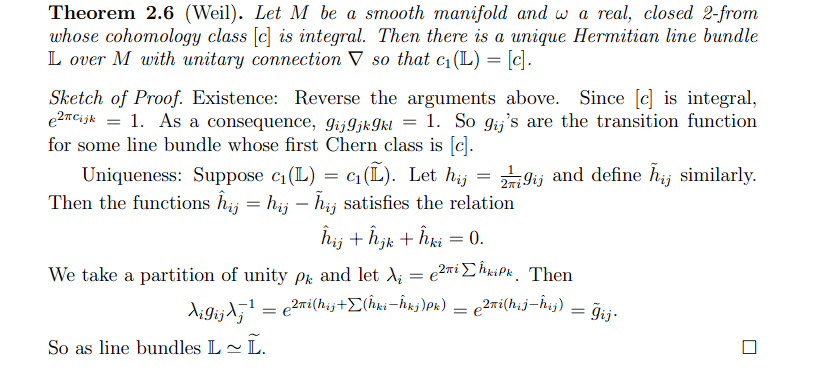
\includegraphics[width=1.0\linewidth]{4.png}
  \caption{Proof}
\end{figure}


